\newpage
\section{Экспериментальная часть}
\subsection{Макет экспериментального стенда}

Макет состоит из спроектированного механического стенда (см. \ref{sec_stand_construction})
и макетной платы Texsas Instruments C2000 Piccolo F28035. В качестве шагового двигателя
используется двигатель, запланированный для работы в реальном приводе - Telco
Motion 4T5618M308 (табл. \ref{engine_params}), в качестве датчика
- импульсный датчик ЛИР-137А 6250-05-ПИ (табл. \ref{encoder_params}).

Функциональная схема макета экспериментального стенда изображена на рис.
\ref{pic_experim_stand_functional_scheme}, где

\begin{itemize}
    \item МК - микроконтроллер
    \item УМ - импульсный усилитель мощности
    \item ШД - шаговой двигатель
    \item ОР - объект регулирования
    \item ДУП - датчик углового положения
    \item ДТ - датчик тока
    \item УТ - усилитель токового сигнала
    \item ДН - датчик напряжения шины питания
    \item ИП - источник питания
\end{itemize}

\begin{figure}
    \centering
    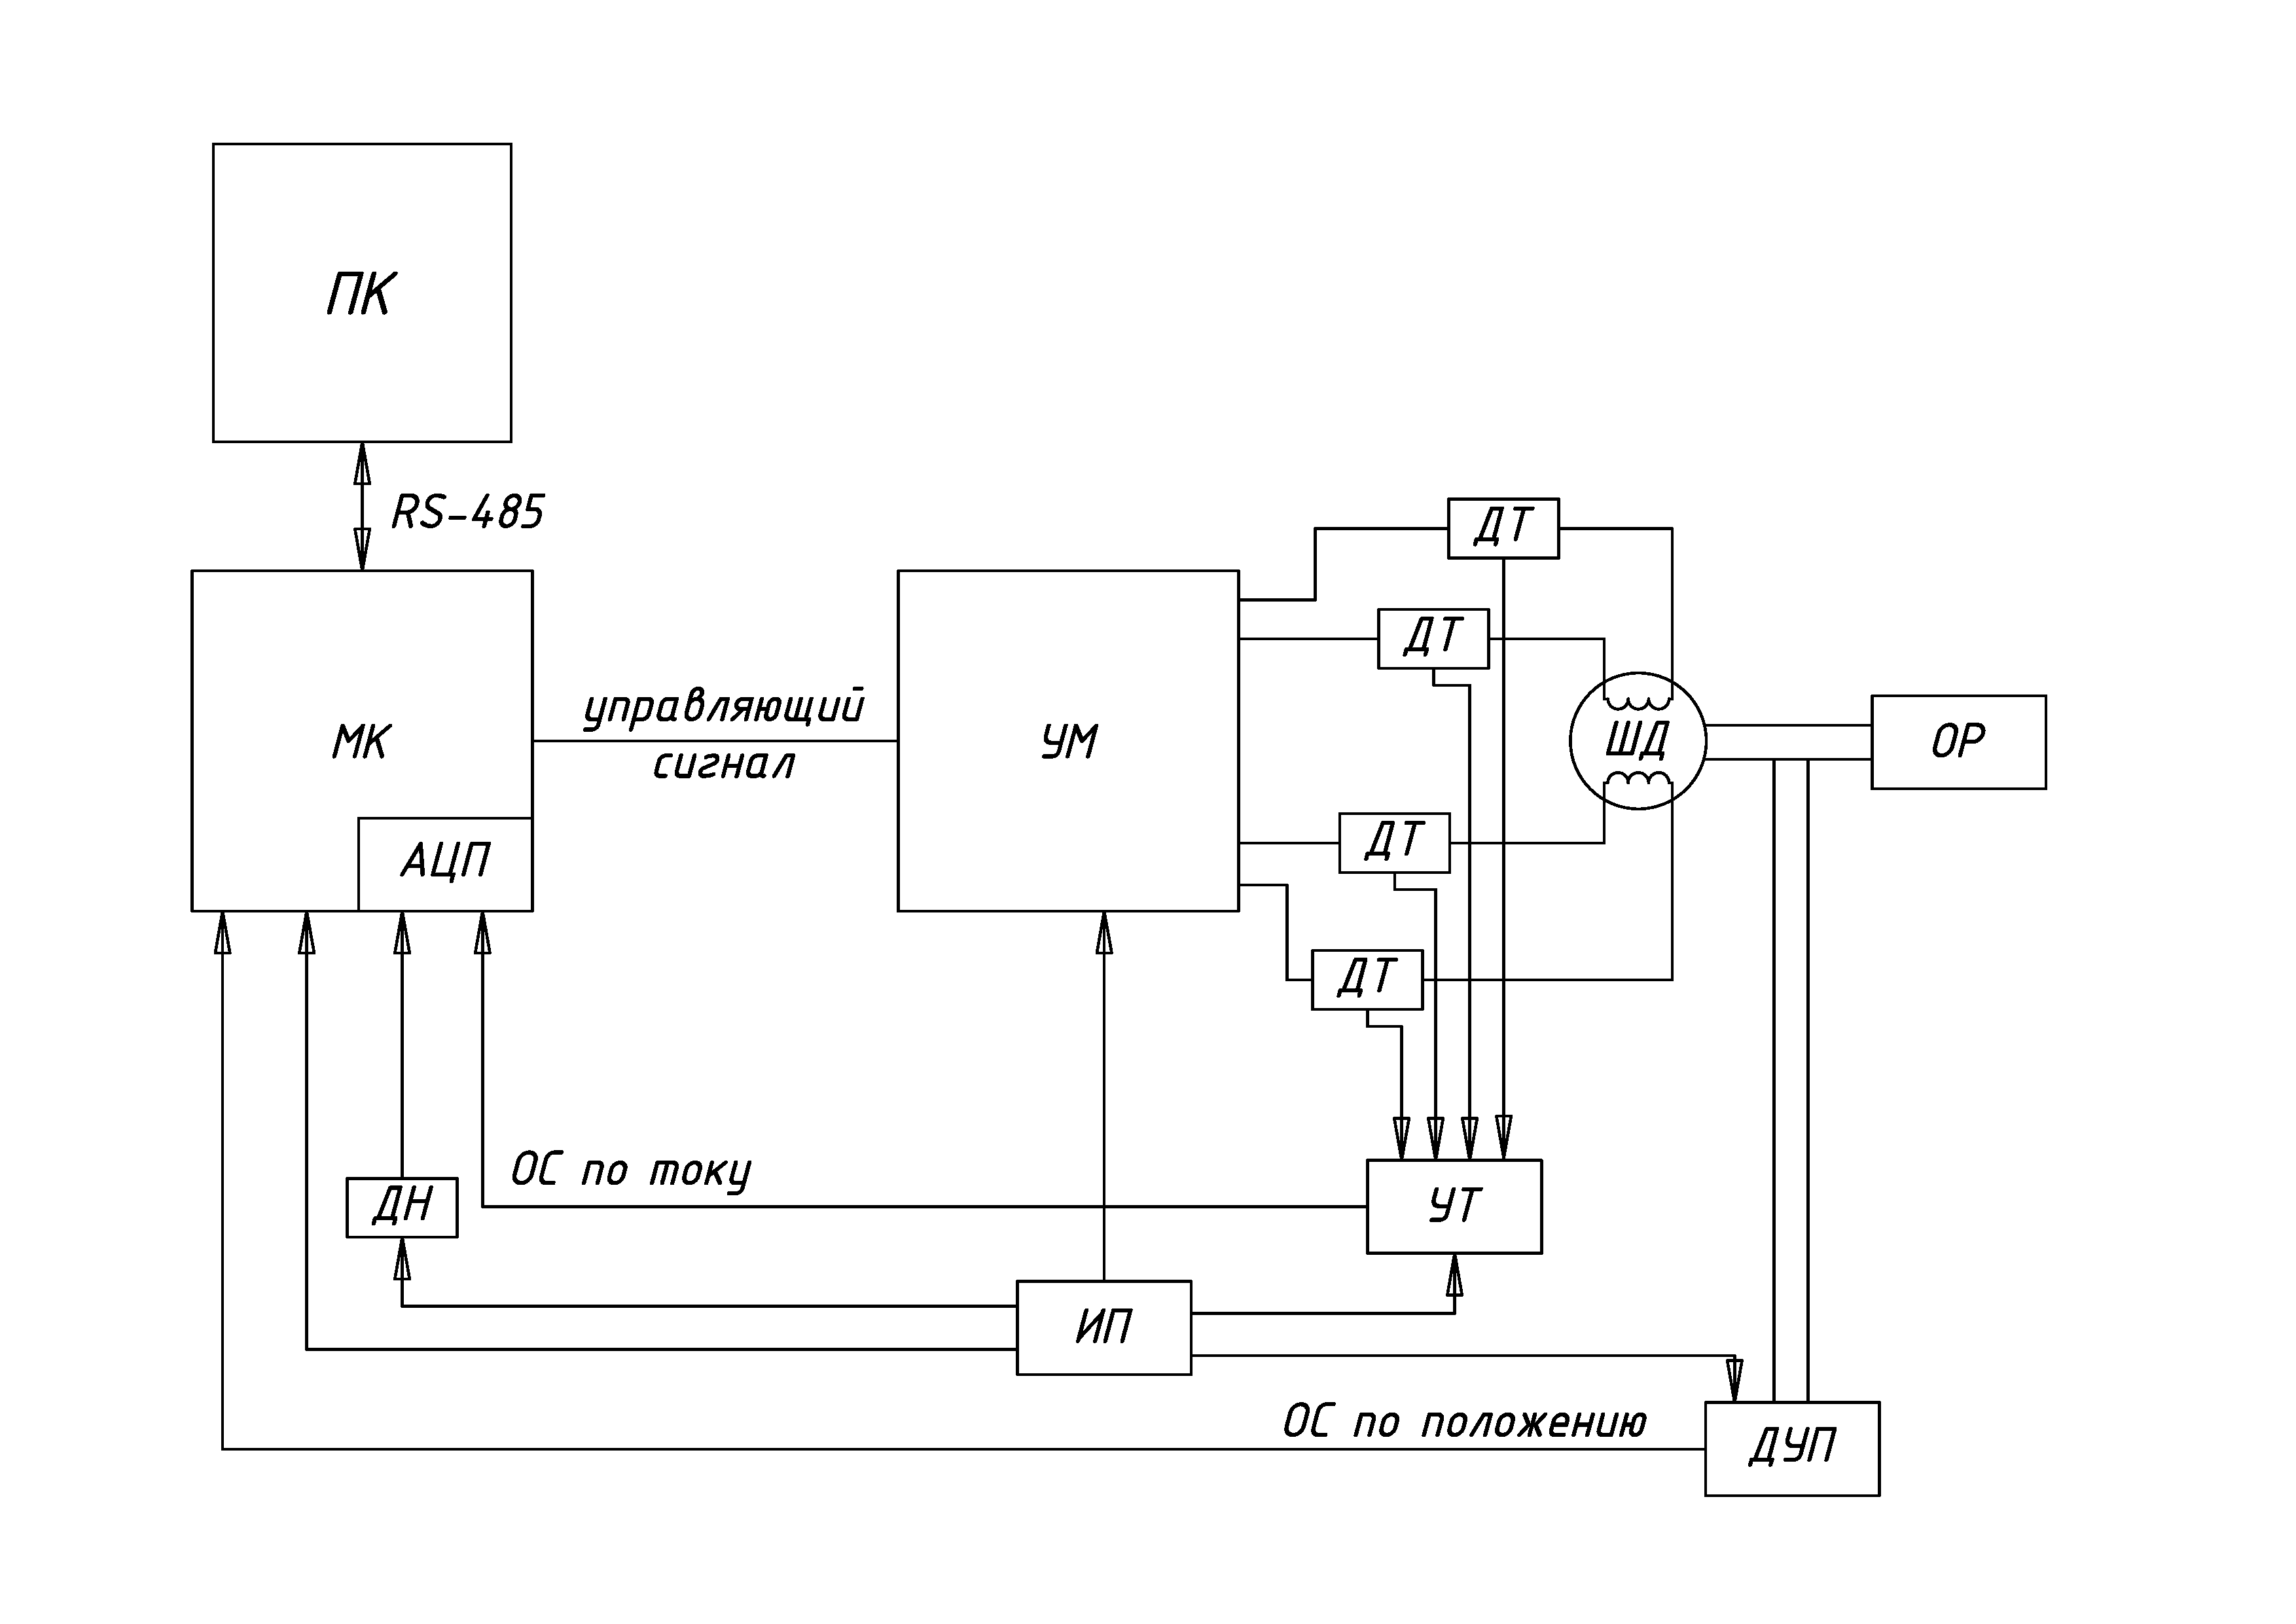
\includegraphics[width=\linewidth, keepaspectratio,
                    clip=true, trim=41mm 31mm 41mm 30mm]
                    {./src/pictures/experim_stand_functional_scheme}
    \caption{Функциональная схема макета экспериментального стенда}
    \label{pic_experim_stand_functional_scheme}
\end{figure}

\subsubsection{Описание экспериментов}

\subsubsection{Результаты экспериментов}

\subsubsection{Выводы по экспериментальной части}
